\documentclass[]{standalone}



\usepackage{lmodern}
\usepackage[T1]{fontenc}
\usepackage{tikz}
\usetikzlibrary{calc,intersections}


\begin{document}

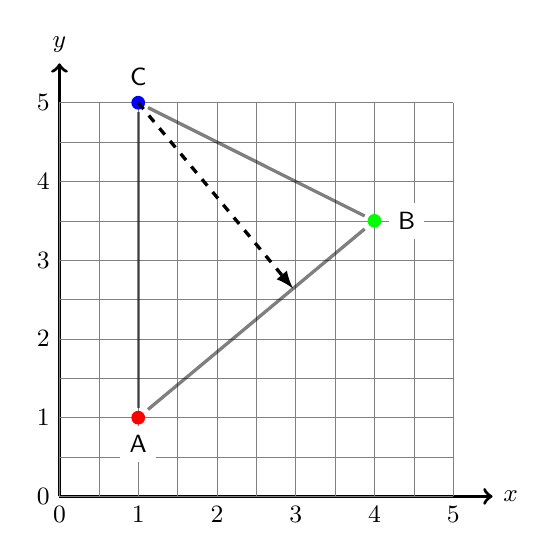
\begin{tikzpicture}[font=\sffamily\small]


	\def \xmax{5};
	\def \ymax{5};
	\def \stepxy{0.5};

	\node[anchor=center, fill=none] (origemXY) at (0,0) {};
	\node[anchor=center, fill=none] (origemX) at (-0.125,0) {};
	\node[anchor=center, fill=none] (origemY) at (0,-0.125) {};
	
	\node[anchor=center] (fimXY) at (\xmax, \ymax) {};
	
	\draw[very thick, ->, anchor=southh west] (origemY) -- (0,\ymax+\stepxy) node(yaxis)[above] {$y$};
	\foreach \y in {0, 1,...,\ymax} \draw (0 cm, \y cm) node[anchor=east]{$\y$};
	
	\draw[very thick, ->, anchor=north west] (origemX) -- (\xmax+\stepxy, 0) node(xaxis)[right] {$x$};
	\foreach \x in {0,1,...,\xmax} \draw (\x cm, 0 cm) node[anchor=north]{$\x$};
    
    % grid
    \draw[style=help lines,step=\stepxy cm] (origemXY) grid (\xmax, \ymax);
    
    
    % points
    \filldraw[red] (1,1) circle (0.08cm) node (A) {} node[anchor=north,fill=white,yshift=-0.1cm, text=black] {A};
   
    \filldraw[green] (4,3.5) circle (0.08cm) node (B) {} node[anchor=west,fill=white,xshift=5pt, text=black] {B};
    \filldraw[blue] (1,5) circle (0.08cm) node (C) {} node[anchor=south,fill=white,yshift=0.1cm, text=black] {C};

     \draw[name path=diagonal1,very thick, opacity=0.5] (A) -- (B);
     \draw[name path=diagonal2,very thick, opacity=0.5] (B) -- (C);
     \draw[name path=diagonal3,very thick, opacity=0.5] (C) -- (A);
     
     \draw[->,>=latex,very thick,dashed] (C.center) -- ($(A)!(C)!(B)$);
     
     %\path[name path=line1] (C) -- +(-3,0);
     
    % \draw[thick,blue,name intersections={of=diagonal and line1,by={Int1}}] (C) -- (Int1);

\end{tikzpicture}

\end{document}
